% This template has been tested with LLNCS DOCUMENT CLASS -- version 2.19 (04-Sep-2017)

% !TeX spellcheck = en-US
% !TeX encoding = utf8
% !TeX program = pdflatex
% !BIB program = bibtex
% -*- coding:utf-8 mod:LaTeX -*-

%"runningheads" enables:
%  - page number on page 2 onwards
%  - title/authors on even/odd pages
%This is good for other readers to enable proper archiving among other papers and pointing to
%content. Even if the title page states the title, when printed and stored in a folder, when
%blindly opening the folder, one could hit not the title page, but an arbitrary page. Therefore,
%it is good to have title printed on the pages, too.
\documentclass[runningheads,a4paper]{llncs}[2017/09/04]

%% If you need packages for other papers,
%% START COPYING HERE

% Set English as language and allow to write hyphenated"=words
%
% Even though `american`, `english` and `USenglish` are synonyms for babel package (according to https://tex.stackexchange.com/questions/12775/babel-english-american-usenglish), the llncs document class is prepared to avoid the overriding of certain names (such as "Abstract." -> "Abstract" or "Fig." -> "Figure") when using `english`, but not when using the other 2.
% english has to go last to set it as default language
\usepackage[ngerman,english]{babel}
%Hint by http://tex.stackexchange.com/a/321066/9075 -> enable "= as dashes
\addto\extrasenglish{\languageshorthands{ngerman}\useshorthands{"}}
\usepackage{algorithm}
\usepackage[noend]{algpseudocode}
\usepackage{ifluatex}
\ifluatex
  \usepackage{fontspec}
  \usepackage[english]{selnolig}
\fi

\iftrue % use default-font
  \ifluatex
    % use the better (sharper, ...) Latin Modern variant of Computer Modern
    \setmainfont{Latin Modern Roman}
    \setsansfont{Latin Modern Sans}
    \setmonofont{Latin Modern Mono} % "variable=false"
    %\setmonofont{Latin Modern Mono Prop} % "variable=true"
  \else
    % better font, similar to the default springer font
    % cfr-lm is preferred over lmodern. Reasoning at http://tex.stackexchange.com/a/247543/9075
    \usepackage[%
      rm={oldstyle=false,proportional=true},%
      sf={oldstyle=false,proportional=true},%
      tt={oldstyle=false,proportional=true,variable=false},%
      qt=false%
    ]{cfr-lm}
  \fi
\else
  % In case more space is needed, it is accepted to use Times New Roman
  \ifluatex
    \setmainfont{TeX Gyre Termes}
    \setsansfont[Scale=.9]{TeX Gyre Heros}
    % newtxtt looks good with times, but no equivalent for lualatex found,
    % therefore tried to replace with inconsolata.
    % However, inconsolata does not look good in the context of LNCS ...
    %\setmonofont[StylisticSet={1,3},Scale=.9]{inconsolata}
    % ... thus, we use the good old Latin Modern Mono font for source code.
    \setmonofont{Latin Modern Mono} % "variable=false"
    %\setmonofont{Latin Modern Mono Prop} % "variable=true"
  \else
    % overwrite cmodern with the Times variant
    \usepackage{newtxtext}
    \usepackage{newtxmath}
    \usepackage[zerostyle=b,scaled=.9]{newtxtt}
  \fi
\fi

\ifluatex
\else
  % fontenc and inputenc are not required when using lualatex
  \usepackage[T1]{fontenc}
  \usepackage[utf8]{inputenc} %support umlauts in the input
\fi

\usepackage{graphicx}

% backticks (`) are rendered as such in verbatim environment. See https://tex.stackexchange.com/a/341057/9075 for details.
\usepackage{upquote}

% Nicer tables (\toprule, \midrule, \bottomrule - see example)
\usepackage{booktabs}

%extended enumerate, such as \begin{compactenum}
\usepackage{paralist}
\usepackage[section]{placeins}
%put figures inside a text
%\usepackage{picins}
%use
%\piccaptioninside
%\piccaption{...}
%\parpic[r]{\includegraphics ...}
%Text...

% For easy quotations: \enquote{text}
% This package is very smart when nesting is applied, otherwise textcmds (see below) provides a shorter command
\usepackage{csquotes}

% For even easier quotations: \qq{text}
\usepackage{textcmds}

%enable margin kerning
\RequirePackage[%
  babel,%
  final,%
  expansion=alltext,%
  protrusion=alltext-nott]{microtype}%
% \texttt{test -- test} keeps the "--" as "--" (and does not convert it to an en dash)
\DisableLigatures{encoding = T1, family = tt* }

%tweak \url{...}
\usepackage{url}
%\urlstyle{same}
%improve wrapping of URLs - hint by http://tex.stackexchange.com/a/10419/9075
\makeatletter
\g@addto@macro{\UrlBreaks}{\UrlOrds}
\makeatother
%nicer // - solution by http://tex.stackexchange.com/a/98470/9075
%DO NOT ACTIVATE -> prevents line breaks
%\makeatletter
%\def\Url@twoslashes{\mathchar`\/\@ifnextchar/{\kern-.2em}{}}
%\g@addto@macro\UrlSpecials{\do\/{\Url@twoslashes}}
%\makeatother

% Diagonal lines in a table - http://tex.stackexchange.com/questions/17745/diagonal-lines-in-table-cell
% Slashbox is not available in texlive (due to licensing) and also gives bad results. This, we use diagbox
%\usepackage{diagbox}

% Required for package pdfcomment later
\usepackage{xcolor}

% For listings
\usepackage{listings}
\lstset{%
  basicstyle=\ttfamily,%
  columns=fixed,%
  basewidth=.5em,%
  xleftmargin=0.5cm,%
  captionpos=b}%
\renewcommand{\lstlistingname}{List.}
% Fix counter as described at https://tex.stackexchange.com/a/28334/9075
\usepackage{chngcntr}
\AtBeginDocument{\counterwithout{lstlisting}{section}}

% Enable nice comments
\usepackage{pdfcomment}
%
\newcommand{\commentontext}[2]{\colorbox{yellow!60}{#1}\pdfcomment[color={0.234 0.867 0.211},hoffset=-6pt,voffset=10pt,opacity=0.5]{#2}}
\newcommand{\commentatside}[1]{\pdfcomment[color={0.045 0.278 0.643},icon=Note]{#1}}
%
% Compatibality with packages todo, easy-todo, todonotes
\newcommand{\todo}[1]{\commentatside{#1}}
% Compatiblity with package fixmetodonotes
\newcommand{\TODO}[1]{\commentatside{#1}}

% Bibliopgraphy enhancements
%  - enable \cite[prenote][]{ref}
%  - enable \cite{ref1,ref2}
% Alternative: \usepackage{cite}, which enables \cite{ref1, ref2} only (otherwise: Error message: "White space in argument")

% Doc: http://texdoc.net/natbib
\usepackage[%
  square,        % for square brackets
  comma,         % use commas as separators
  numbers,       % for numerical citations;
%  sort,          % orders multiple citations into the sequence in which they appear in the list of references;
  sort&compress, % as sort but in addition multiple numerical citations
                 % are compressed if possible (as 3-6, 15);
]{natbib}
% In the bibliography, references have to be formatted as 1., 2., ... not [1], [2], ...
\renewcommand{\bibnumfmt}[1]{#1.}

\ifluatex
  % does not work when using luatex
  % see: https://tex.stackexchange.com/q/419288/9075
\else
  % Prepare more space-saving rendering of the bibliography
  % Source: https://tex.stackexchange.com/a/280936/9075
  \SetExpansion
  [ context = sloppy,
    stretch = 30,
    shrink = 60,
    step = 5 ]
  { encoding = {OT1,T1,TS1} }
  { }
\fi

% Put footnotes below floats
% Source: https://tex.stackexchange.com/a/32993/9075
\usepackage{stfloats}
\fnbelowfloat

% Enable that parameters of \cref{}, \ref{}, \cite{}, ... are linked so that a reader can click on the number an jump to the target in the document
\usepackage{hyperref}
% Enable hyperref without colors and without bookmarks
\hypersetup{hidelinks,
  colorlinks=true,
  allcolors=black,
  pdfstartview=Fit,
  breaklinks=true}
%
% Enable correct jumping to figures when referencing
\usepackage[all]{hypcap}

\usepackage[group-four-digits,per-mode=fraction]{siunitx}

%enable \cref{...} and \Cref{...} instead of \ref: Type of reference included in the link
\usepackage[capitalise,nameinlink]{cleveref}
%Nice formats for \cref
\crefname{section}{Sect.}{Sect.}
\Crefname{section}{Section}{Sections}
\crefname{listing}{\lstlistingname}{\lstlistingname}
\Crefname{listing}{Listing}{Listings}

%Intermediate solution for hyperlinked refs. See https://tex.stackexchange.com/q/132420/9075 for more information.
\newcommand{\Vlabel}[1]{\label[line]{#1}\hypertarget{#1}{}}
\newcommand{\lref}[1]{\hyperlink{#1}{\FancyVerbLineautorefname~\ref*{#1}}}

\usepackage{xspace}
%\newcommand{\eg}{e.\,g.\xspace}
%\newcommand{\ie}{i.\,e.\xspace}
\newcommand{\eg}{e.\,g.,\ }
\newcommand{\ie}{i.\,e.,\ }

%introduce \powerset - hint by http://matheplanet.com/matheplanet/nuke/html/viewtopic.php?topic=136492&post_id=997377
\DeclareFontFamily{U}{MnSymbolC}{}
\DeclareSymbolFont{MnSyC}{U}{MnSymbolC}{m}{n}
\DeclareFontShape{U}{MnSymbolC}{m}{n}{
  <-6>    MnSymbolC5
  <6-7>   MnSymbolC6
  <7-8>   MnSymbolC7
  <8-9>   MnSymbolC8
  <9-10>  MnSymbolC9
  <10-12> MnSymbolC10
  <12->   MnSymbolC12%
}{}
\DeclareMathSymbol{\powerset}{\mathord}{MnSyC}{180}

\ifluatex
\else
  % Enable copy and paste - also of numbers
  % This has to be done instead of \usepackage{cmap}, because it does not work together with cfr-lm.
  % See: https://tex.stackexchange.com/a/430599/9075
  \input glyphtounicode
  \pdfgentounicode=1
\fi

% correct bad hyphenation here
\hyphenation{op-tical net-works semi-conduc-tor}

%% END COPYING HERE


% Add copyright
% Do that for the final version or if you send it to colleagues
\iffalse
  %state: intended|submitted|llncs
  %you can add "crop" if the paper should be cropped to the format Springer is publishing
  \usepackage[intended]{llncsconf}

  \conference{name of the conference}

  %in case of "llncs" (final version!)
  %example: llncs{Anonymous et al. (eds). \emph{Proceedings of the International Conference on \LaTeX-Hacks}, LNCS~42. Some Publisher, 2016.}{0042}
  \llncs{book editors and title}{0042} %% 0042 is the start page
\fi

% For demonstration purposes only
\usepackage[math]{blindtext}
\usepackage{mwe}
\raggedbottom

\begin{document}

\title{Security Analysis of Bitcoin Transactions through Statistical Graph Annotation}
%If Title is too long, use \titlerunning
\titlerunning{6000D Project Report}

%Single insitute
\author{Pranav A \and Chun Sik Chan}
%If there are too many authors, use \authorrunning
%\authorrunning{First Author et al.}
\institute{Big Data Institute, HKUST}

%% Multiple insitutes - ALTERNATIVE to the above
% \author{%
%     Firstname Lastname\inst{1} \and
%     Firstname Lastname\inst{2}
% }
%
%If there are too many authors, use \authorrunning
%  \authorrunning{First Author et al.}
%
%  \institute{
%      Insitute 1\\
%      \email{...}\and
%      Insitute 2\\
%      \email{...}
%}

\maketitle

\begin{abstract}
  Money transaction using bitcoin is getting prevalent these days due
  to its government-free, secure, decentralized and open-sourced design. It has been exploited for money laundering. However, it is still possible to detect some trail by analysing the structure of the transaction network. This paper aims to construct a user transaction flow graph of bitcoins and analyze the security and networking properties.
  By developing basic heuristics, we bundled the public keys of the users
  from the transaction graph into the user bitcoin flow graph. In a case study of the Silk Road arrest, we demonstrated how coin-mixing trails could be discovered using the user flow graph.
\end{abstract}

\section{Introduction}

Anonymity and fungibility are the key characteristics of any financial transaction system. Bitcoin architecture aims for these characteristics through transparency and privacy. Bitcoin assigns pseudonyms to the entities. Here, by entities, we mean, users, wallets, and organizations. These entities are represented by the public keys or addresses. It should be noted that information regarding public keys of senders and receivers, and transaction values are made available to the public. However, it is unknown which public keys belong to which entity. A user can be thought of as a mapping of a set of public keys.
 
The main focus of this project is to discover this mapping and construct a networking graph through those mappings. Generally, this is achieved through clustering. Firstly, we parse the blockchain and construct a transaction graph. From that transaction graph, we apply our multi-input heuristic. This is a fact that all inputs involved in the multi-input transaction represent the same wallet. This heuristic allows us to create a user graph. Through this user graph, we do some statistical analysis to gather more insights on the bitcoin network. Finally, we provide a case study on Silk Road arrest \cite{anderson_farivar_2013}. We demonstrate how a trail could be discovered using graph search algorithms. We have proposed our own algorithms for blockchain parsing and graph creation, which are a lot more memory-efficient.

\section{Related Work}

This section discusses some pros and cons of the previous work done on multi-input heuristic and transaction graph analysis for the blockchain.
In the seminal Bitcoin paper \cite{nakamoto2008bitcoin}, Satoshi introduced the multi-input heuristic, which basically implies that all transaction inputs would correspond to the identical wallet.
Fleder et al. \cite{fleder2015bitcoin} showed that using the multi-input heuristic, one could identify most social-able nodes in the bitcoin graphs using PageRank.
Also with the usage of multi-input heuristic, Reid et al. \cite{reid2013analysis} analyzes the relation between the topological structure of the transaction graphs and user inflow graph.

Besides, multi-input heuristics, there exists some work whose clustering depends on other heuristics.
Ober et al. \cite{ober2013structure} used entity merging to observe structural patterns in the topological networks of the bitcoin structure.
They also analyzed the dormant coins and performed statistical tests to show that they are close to Poisson independent process.
Ermilov et al. \cite{ermilov2017automatic} used blockchain information with off-chain information for clustering. 
Verified information and tags were used as the off-chain information.
This helped in address separation and avoiding errors.
Harrigan et al. \cite{harrigan2016unreasonable} demonstrated the effectiveness of the address clustering in Bitcoin networks.
The reasons include recycling of addresses, slow growth of clusters in the networks, disregarding the merging of clusters and clusters resulting in high degree of centrality.
Dorit et al. \cite{ron2013quantitative} provided a qualitative analysis of the bitcoin transaction graph.
Unfortunately, regarding their title, they did not provide a analysis on "full" graph. 
Also, no information regarding directions for incomplete edges is given.
The construction of graph they proposed is clumsy and requires a lot of parameters.

By analyzing the anonymity risks involved in the bitcoin transactions, Moser et al. \cite{moser2014towards, moser2013inquiry} provided risk analysis and scoring model for the blockchain based businesses. They also provided an in-depth analysis of money laundering tools using reverse engineering.
Nick et al. \cite{nick2015data} substantiated experiments on deanonymization which were data-driven.
They analyzed some performance on clustering heuristics, or in other words, the addresses which refer to the same wallet.
They found a loophole in Connection Bloom Filtering, which was eventually used as a ground truth for verifying the results.
They mentioned that even a strongest peer-to-peer network can be deanonymized using a multi-input heuristic.
On an average, 68.59 \% addresses can be revealed using these heuristics, in addition to other ones as well.
Lischke et al. \cite{lischke2016analyzing} constructed graphical structures based on business distribution, adoption, and geo-locations. However, their construction of networking graphs relied on only one metric, betweenness centrality.

Clearly, none of the work above mention about memory management and dealing with the nodes of the subgraph. In the upcoming sections, we will walkthorough our designs on such algorithms.

\section{Blockchain Parsing}

This section discusses on how to parse the data of the blockchain. We also provide our memory management algorithm, which aids in dealing with big data.

\subsection{Process}

Using the peer-to-peer client, we downloaded the bitcoin blockchain from 2009 to October 2013.
Then we parsed the blockchain into following components.

\begin{enumerate}
	\item Transaction input addresses and output addresses
	\item Transaction hash
	\item Transaction values
	\item Transaction datetime
	\item Block number
\end{enumerate}

The outputs are shown in figure \ref{parse}.

\begin{figure}[!htb]
	\centering 
	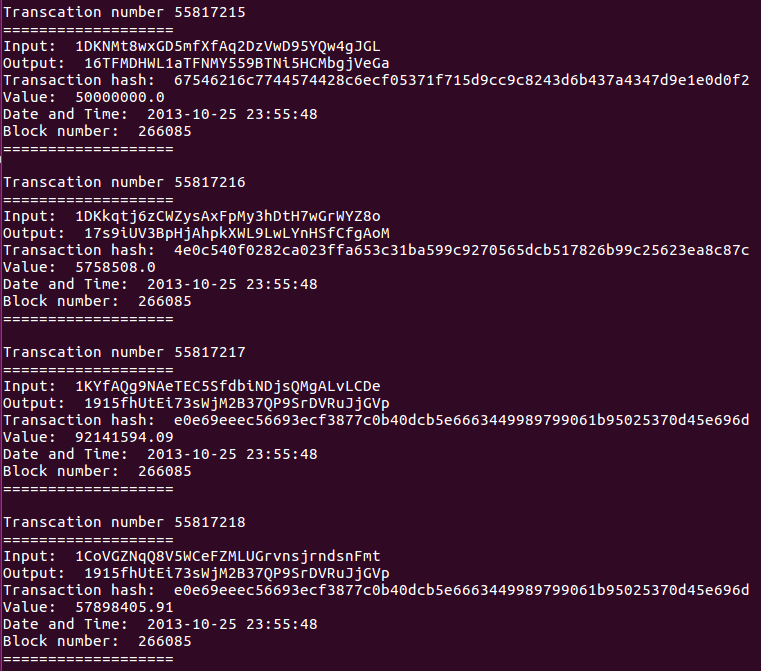
\includegraphics[width=0.8\columnwidth]{parse} 
	\caption{Parsed Blockchain} % The text in the square bracket is the caption for the list of figures while the text in the curly brackets is the figure caption
	\label{parse}
\end{figure}

\subsection{Bottleneck}

The blockchain size grows exponentially every year. Figure \ref{first} and \ref{second} show the size evolution of blockchain.
A bitcoin transaction contains inputs and outputs.
The input contains the hash of the previous transaction and an index of the corresponding output.
The output contains the public addresses of receivers, transaction amount and the public addresses of the sender are missing in the current transaction.
It's very essential to keep the outputs of the previous transaction.


\begin{figure}[!htb]
	\centering 
	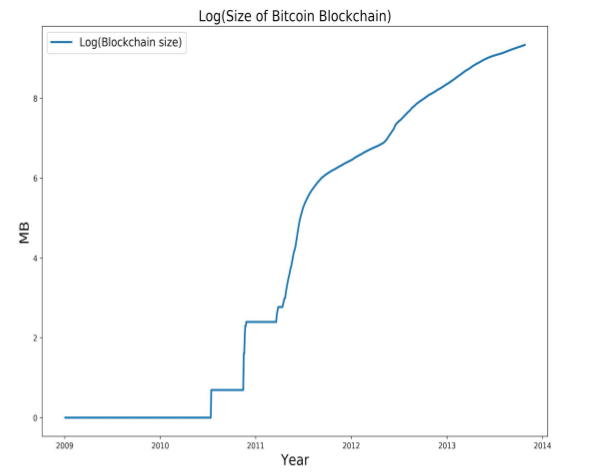
\includegraphics[width=0.8\columnwidth]{1} 
	\caption{Yearwise comparision of Blockchain size} % The text in the square bracket is the caption for the list of figures while the text in the curly brackets is the figure caption
	\label{first}
\end{figure}

\begin{figure}[!htb]
	\centering 
	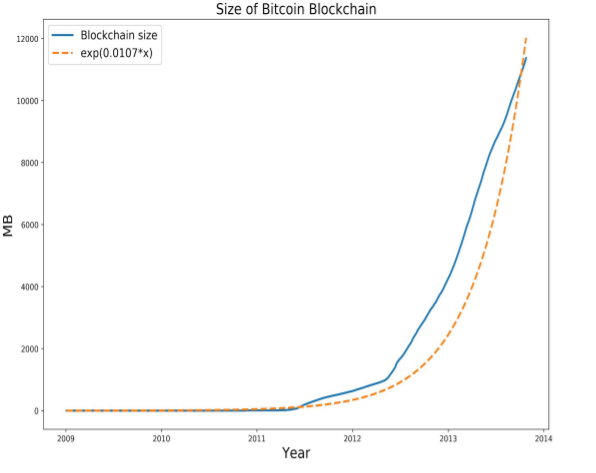
\includegraphics[width=0.8\columnwidth]{2} 
	\caption{Yearwise comparision of Blockchain size} % The text in the square bracket is the caption for the list of figures while the text in the curly brackets is the figure caption
	\label{second}
\end{figure}

Hence, we created an algorithm to manage this huge parsed blockchain data, shown in Algorithm 1.

\begin{algorithm}[!h]
	\caption{Bitcoin Blockchain Parsing with O(len(blocks)) memory usage}
	\begin{algorithmic}
		\State \textbf{Input: } Bitcoin transactions $T$, the end time $e_t$, and a empty file $F$.
		\State Let $H(.)$ be a hash table pointing to memory
		\For {each $tx$ in $T$}
		\If {$tx.time > e_t$}
		\State return
		\EndIf
		\If {$tx$ is a coinbase transaction}
		\State skip
		\EndIf
		\State $H(tx.hash) \gets tx.outputs$
		\State $\texttt{total_value} \gets$ sum of the values in all valid outputs of tx
		\For {each $o$ in $tx.outputs$}
		\For {each $i$ in $tx.inputs$}
		\State sender $\gets$ the address of the sender retrieved from $H(i.hash)[i.index]$
		\State $recepient \gets o.address$
		\State Write to F: $sender, recepient, o.value / total_{value}, tx.hash, tx.time$
		\State Remove $H(i.hash)[i.index]$ from $H(i.hash)$
		\If {$H(i.hash)$ is empty}
		\State Remove $H(i.hash)$ from $H$
		\EndIf
		\EndFor
		\EndFor
		\EndFor
		\State \textbf{Output: } The parsed data $F$
	\end{algorithmic}
\end{algorithm}

For processing the algorithm 1, we used Azure virtual machine with 2 virtual CPUs and 32 GB memory.
The performance is shown in figure 1.

\begin{figure}[!htb]
	\centering 
	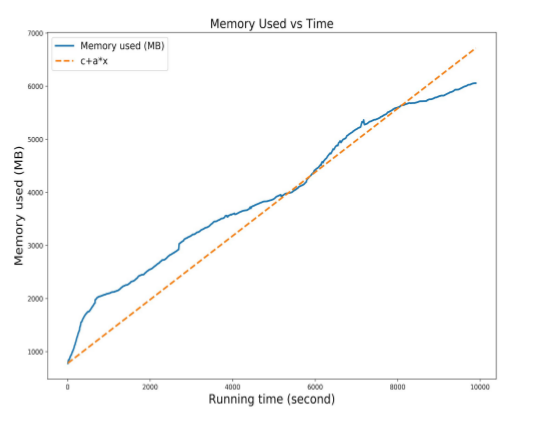
\includegraphics[width=0.8\columnwidth]{size} 
	\caption{Performance of Memory Management Algorithm} % The text in the square bracket is the caption for the list of figures while the text in the curly brackets is the figure caption
	\label{size}
\end{figure}


\section{Graph Annotation}

Once the blockchain data is parsed, we follow-up by creating a transaction graph flow.

Here, each node is a public key appeared in the outputs or inputs of a transaction.
Each edge is transaction information including the transaction hash, value, datetime, and block number.

\begin{figure}[!htb]
	\centering 
	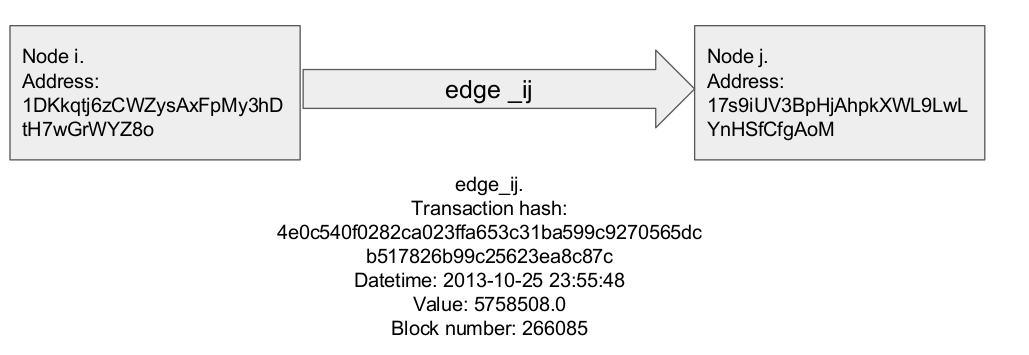
\includegraphics[width=0.8\columnwidth]{graph} 
	\caption{Data Structure of the Transaction Graph} % The text in the square bracket is the caption for the list of figures while the text in the curly brackets is the figure caption
	\label{graph}
\end{figure}

The data structure of the transaction graph is shown in \ref{graph}.

Usually a real world entity owns more than one address. We are interested in the transaction activities of the entity It is feasible to link addresses in blockchain based assumption:
The input addresses of the same transaction belong to the same real world entity.
Our algorithm on linking related public addresses is shown in algorithm 2.

\begin{algorithm}[!h]
	\caption{Linking Related Public Addresses}
	\begin{algorithmic}
		\State \textbf{Input: } Transactions between public addresses $T$
		\State $G \gets$ An empty undirected graph
		\State $X \gets$ The set of the hashes in $T$
		\For {each hash $h$ in $X$}
		\State $S \gets$ Find the set of sender addresses in the transactions of hash $h$
		\State $N \gets$ Size of $S$
		\For {$i=0$ to $N-2$}
		\State Add $(S[i], S[i+1])$ as an edge to $G$
		\EndFor
		\EndFor
		\State $C \gets$ Find the set of all connect components of $G$
		\State \textbf{Output: } 
		\State 1. Mapping U2A: $i \rightarrow i^{th} set \in C$
		\State 2. Mapping A2U: a public address$ p \gets$ the index of the connected component in $C$ which contains $p$
	\end{algorithmic}
\end{algorithm}

After linking user addresses, the objective is to construct a user graph which shows flow of transactions from users. 
The data structure of the figure is shown in \ref{trans}.

\begin{figure}[!htb]
	\centering 
	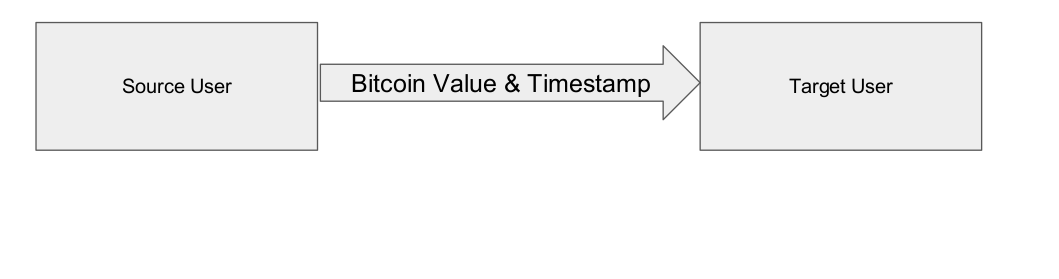
\includegraphics[width=0.8\columnwidth]{trans} 
	\caption{Data Structure of the User Graph} % The text in the square bracket is the caption for the list of figures while the text in the curly brackets is the figure caption
	\label{trans}
\end{figure}

Initially we constructed a trivial imperfect graph depicting through the public keys.
It’s usually considered a good practice to generate a new public key for every transaction.
Hence, we need some heuristics to bundle these public keys together for a user.
We constructed a supplementary graph which analyzes the relation between transactions inputs / outputs and public keys.

\subsection{Bundling addresses into a user}

For the supplementary graph, we represent a vertex with a public key.
We constructed an undirected edge between the vertices which are the inputs to the same transaction.
Each maximal connected subgraph would correspond to a single user.

In order to discover maximal connected subgraphs, we used Depth-First search to discover such components. 
Since, one vertex could lie in only one component, we picked seed nodes randomly. From that seed node, we traversed all the connected public keys and bundled them together into one user.

This is a complex process to understand. Hence, we have provdied a series of figures (\ref{a1}, \ref{a2}, \ref{a3}) to understand graph annotation.

\begin{figure}[!htb]
	\centering 
	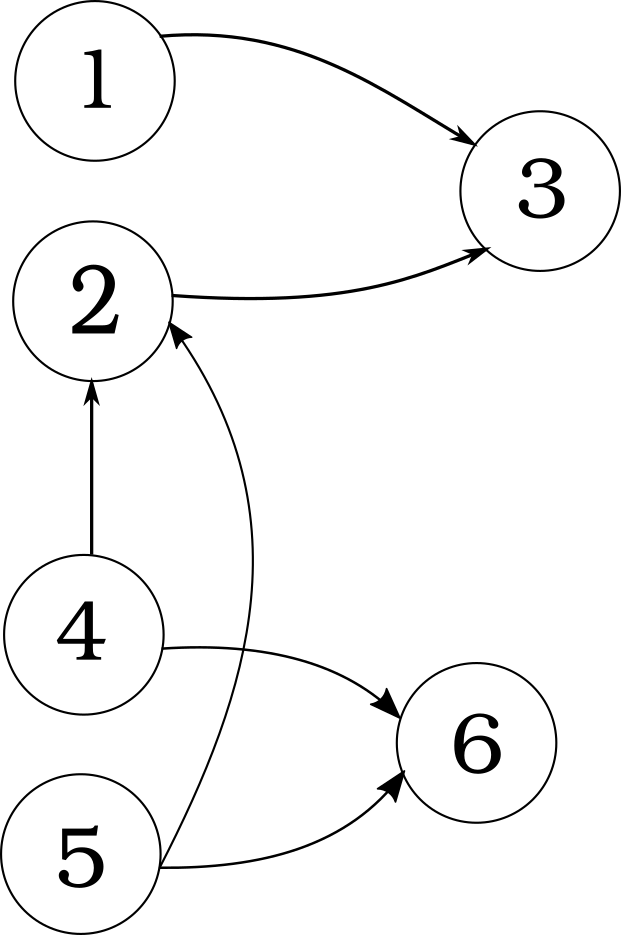
\includegraphics[width=0.4\columnwidth]{bitmap} 
	\caption{The figure shows the flow graph of the transaction graph as mentioned earlier. Note that this is only a subgraph from the larger network.} % The text in the square bracket is the caption for the list of figures while the text in the curly brackets is the figure caption
	\label{a1}
\end{figure}

\begin{figure}[!htb]
	\centering 
	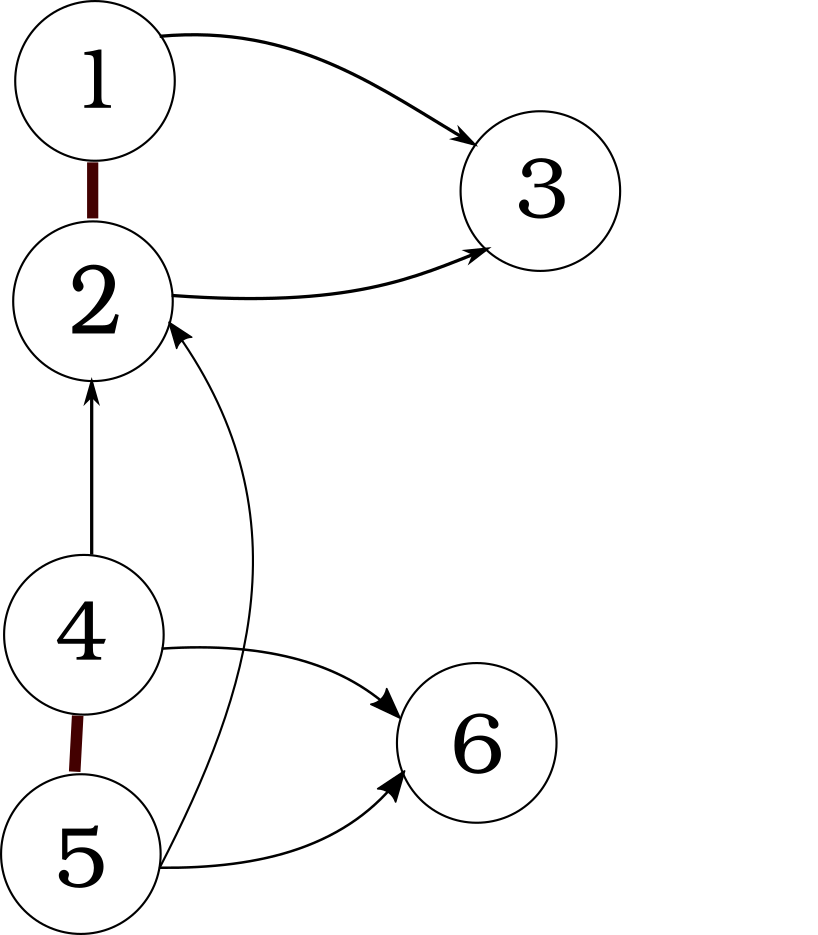
\includegraphics[width=0.4\columnwidth]{bitmap1} 
	\caption{We bundled 1 and 2 together because they were the inputs for the transaction to 3. Hence, we join 1 and 2 by a undirected edge.Similarly it goes for 4 and 5.} % The text in the square bracket is the caption for the list of figures while the text in the curly brackets is the figure caption
	\label{a2}
\end{figure}

\begin{figure}[!htb]
	\centering 
	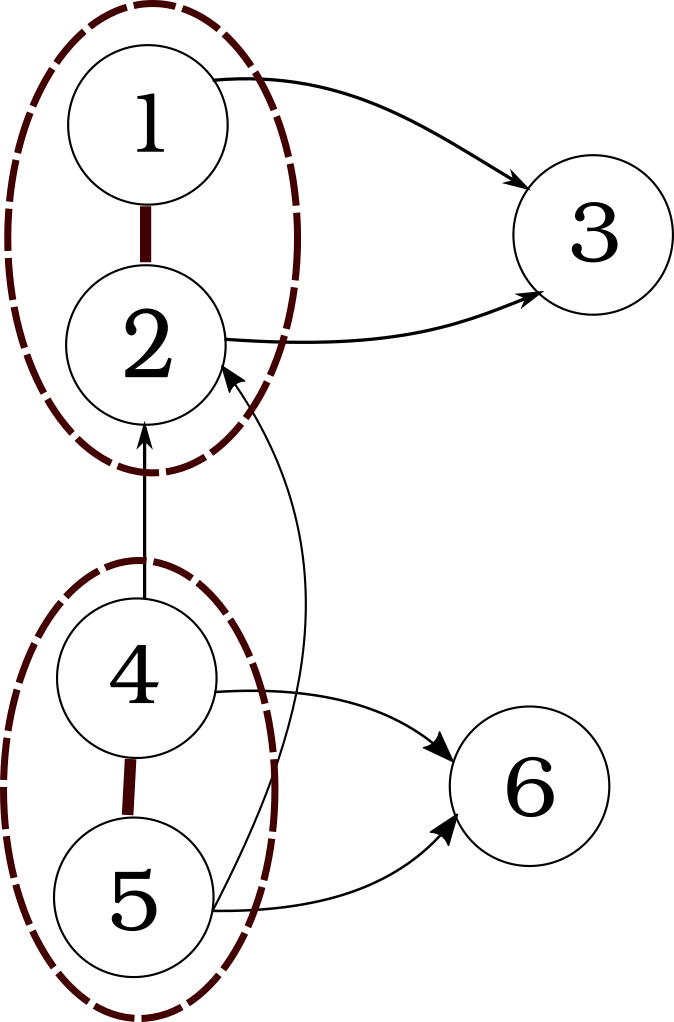
\includegraphics[width=0.4\columnwidth]{bitmap2} 
	\caption{Now, we only analyze the undirected edges. We extract the maximal connected component and annotate that component as a user.} % The text in the square bracket is the caption for the list of figures while the text in the curly brackets is the figure caption
	\label{a3}
\end{figure}

Our graph will concur some missing and corrupted data due to our heuristic assumptions and partial blockchain analysis.
Hence, we remove the outliers in following ways:
\begin{enumerate}
	\item Remove the transactions where the algorithm was not able to bundle the public keys into users.
	\item Remove the isolated components and self-loops.
\end{enumerate}

\begin{figure}[h]
	\centering 
	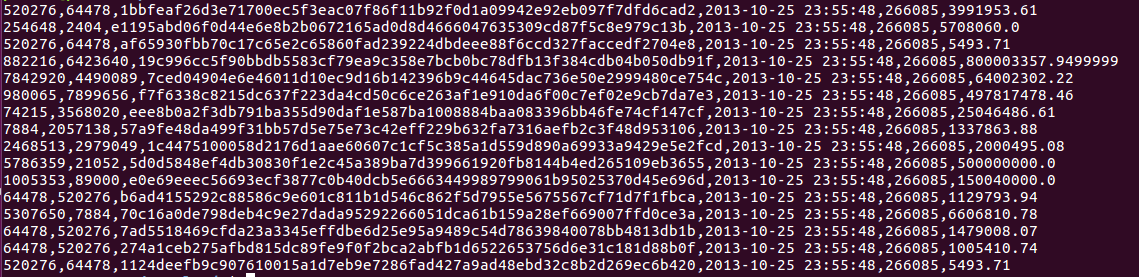
\includegraphics[width=\columnwidth]{final} 
	\caption{The final graph of the trasactions between the users is represented like this.} % The text in the square bracket is the caption for the list of figures while the text in the curly brackets is the figure caption
	\label{final}
\end{figure}


\subsection{Analysis on the user graphs}

We draw a log-log plot of degree distribution which is shown \ref{degree}. 
It shows that the graph slightly deviates from power law.

\begin{figure}[h]
	\centering 
	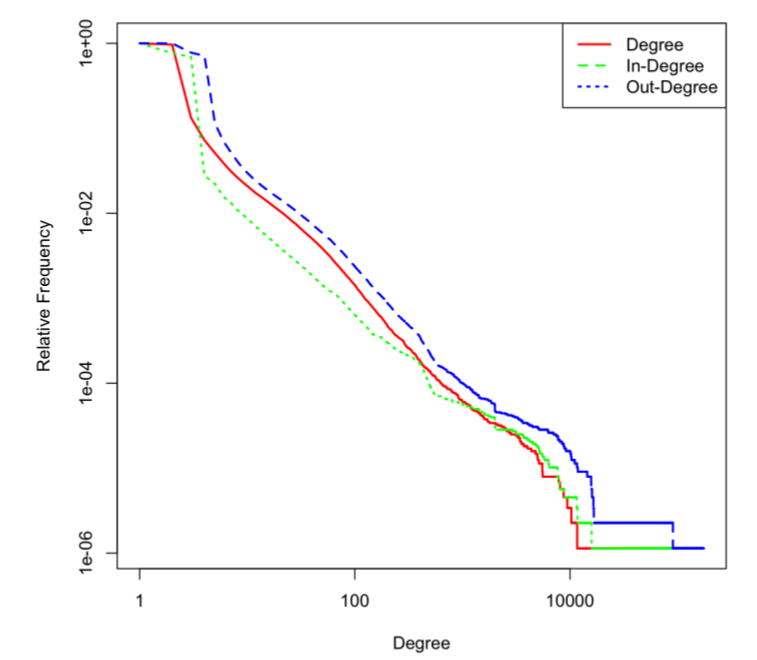
\includegraphics[width=0.8\columnwidth]{degree} 
	\caption{Degree Distribution of the user graph} % The text in the square bracket is the caption for the list of figures while the text in the curly brackets is the figure caption
	\label{degree}
\end{figure}

We applied goodness of fit to our curve and found the p-value to be greater than threshold.
This proves that bitcoin transactions do not follow preferential attachment and it is not a scale-free network. This is mainly due to decentralized architecture of Bitcoin.

The plot of component size distribution is shown in figure \ref{comp}. Clearly, this does not follow power law as well.

\begin{figure}[h]
	\centering 
	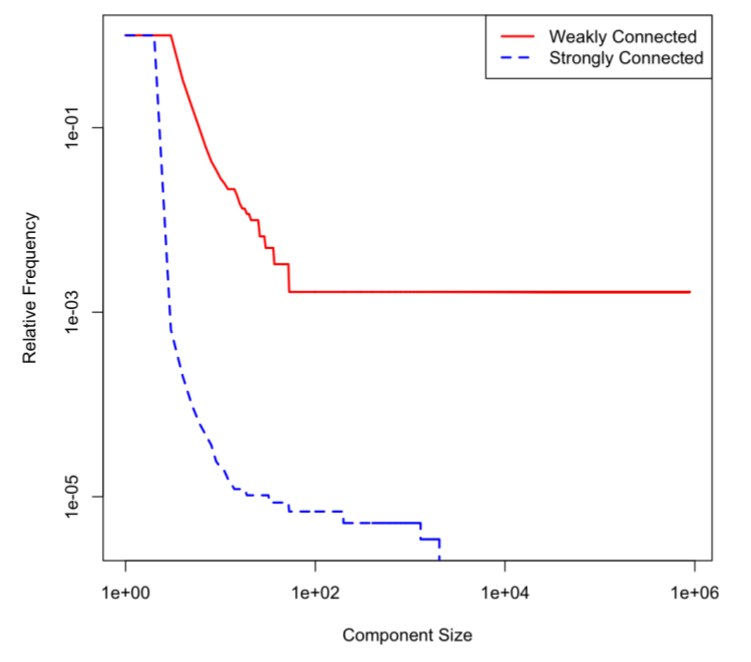
\includegraphics[width=0.8\columnwidth]{comp} 
	\caption{Component Size Distribution of the user graph} % The text in the square bracket is the caption for the list of figures while the text in the curly brackets is the figure caption
	\label{comp}
\end{figure}

We found that most of the nodes with high in-degree and out-degree were from gambling websites like SatoshiDICE.

The visualization of the user graph is shown in figure \ref{viz}.


\begin{figure}[h]
	\centering 
	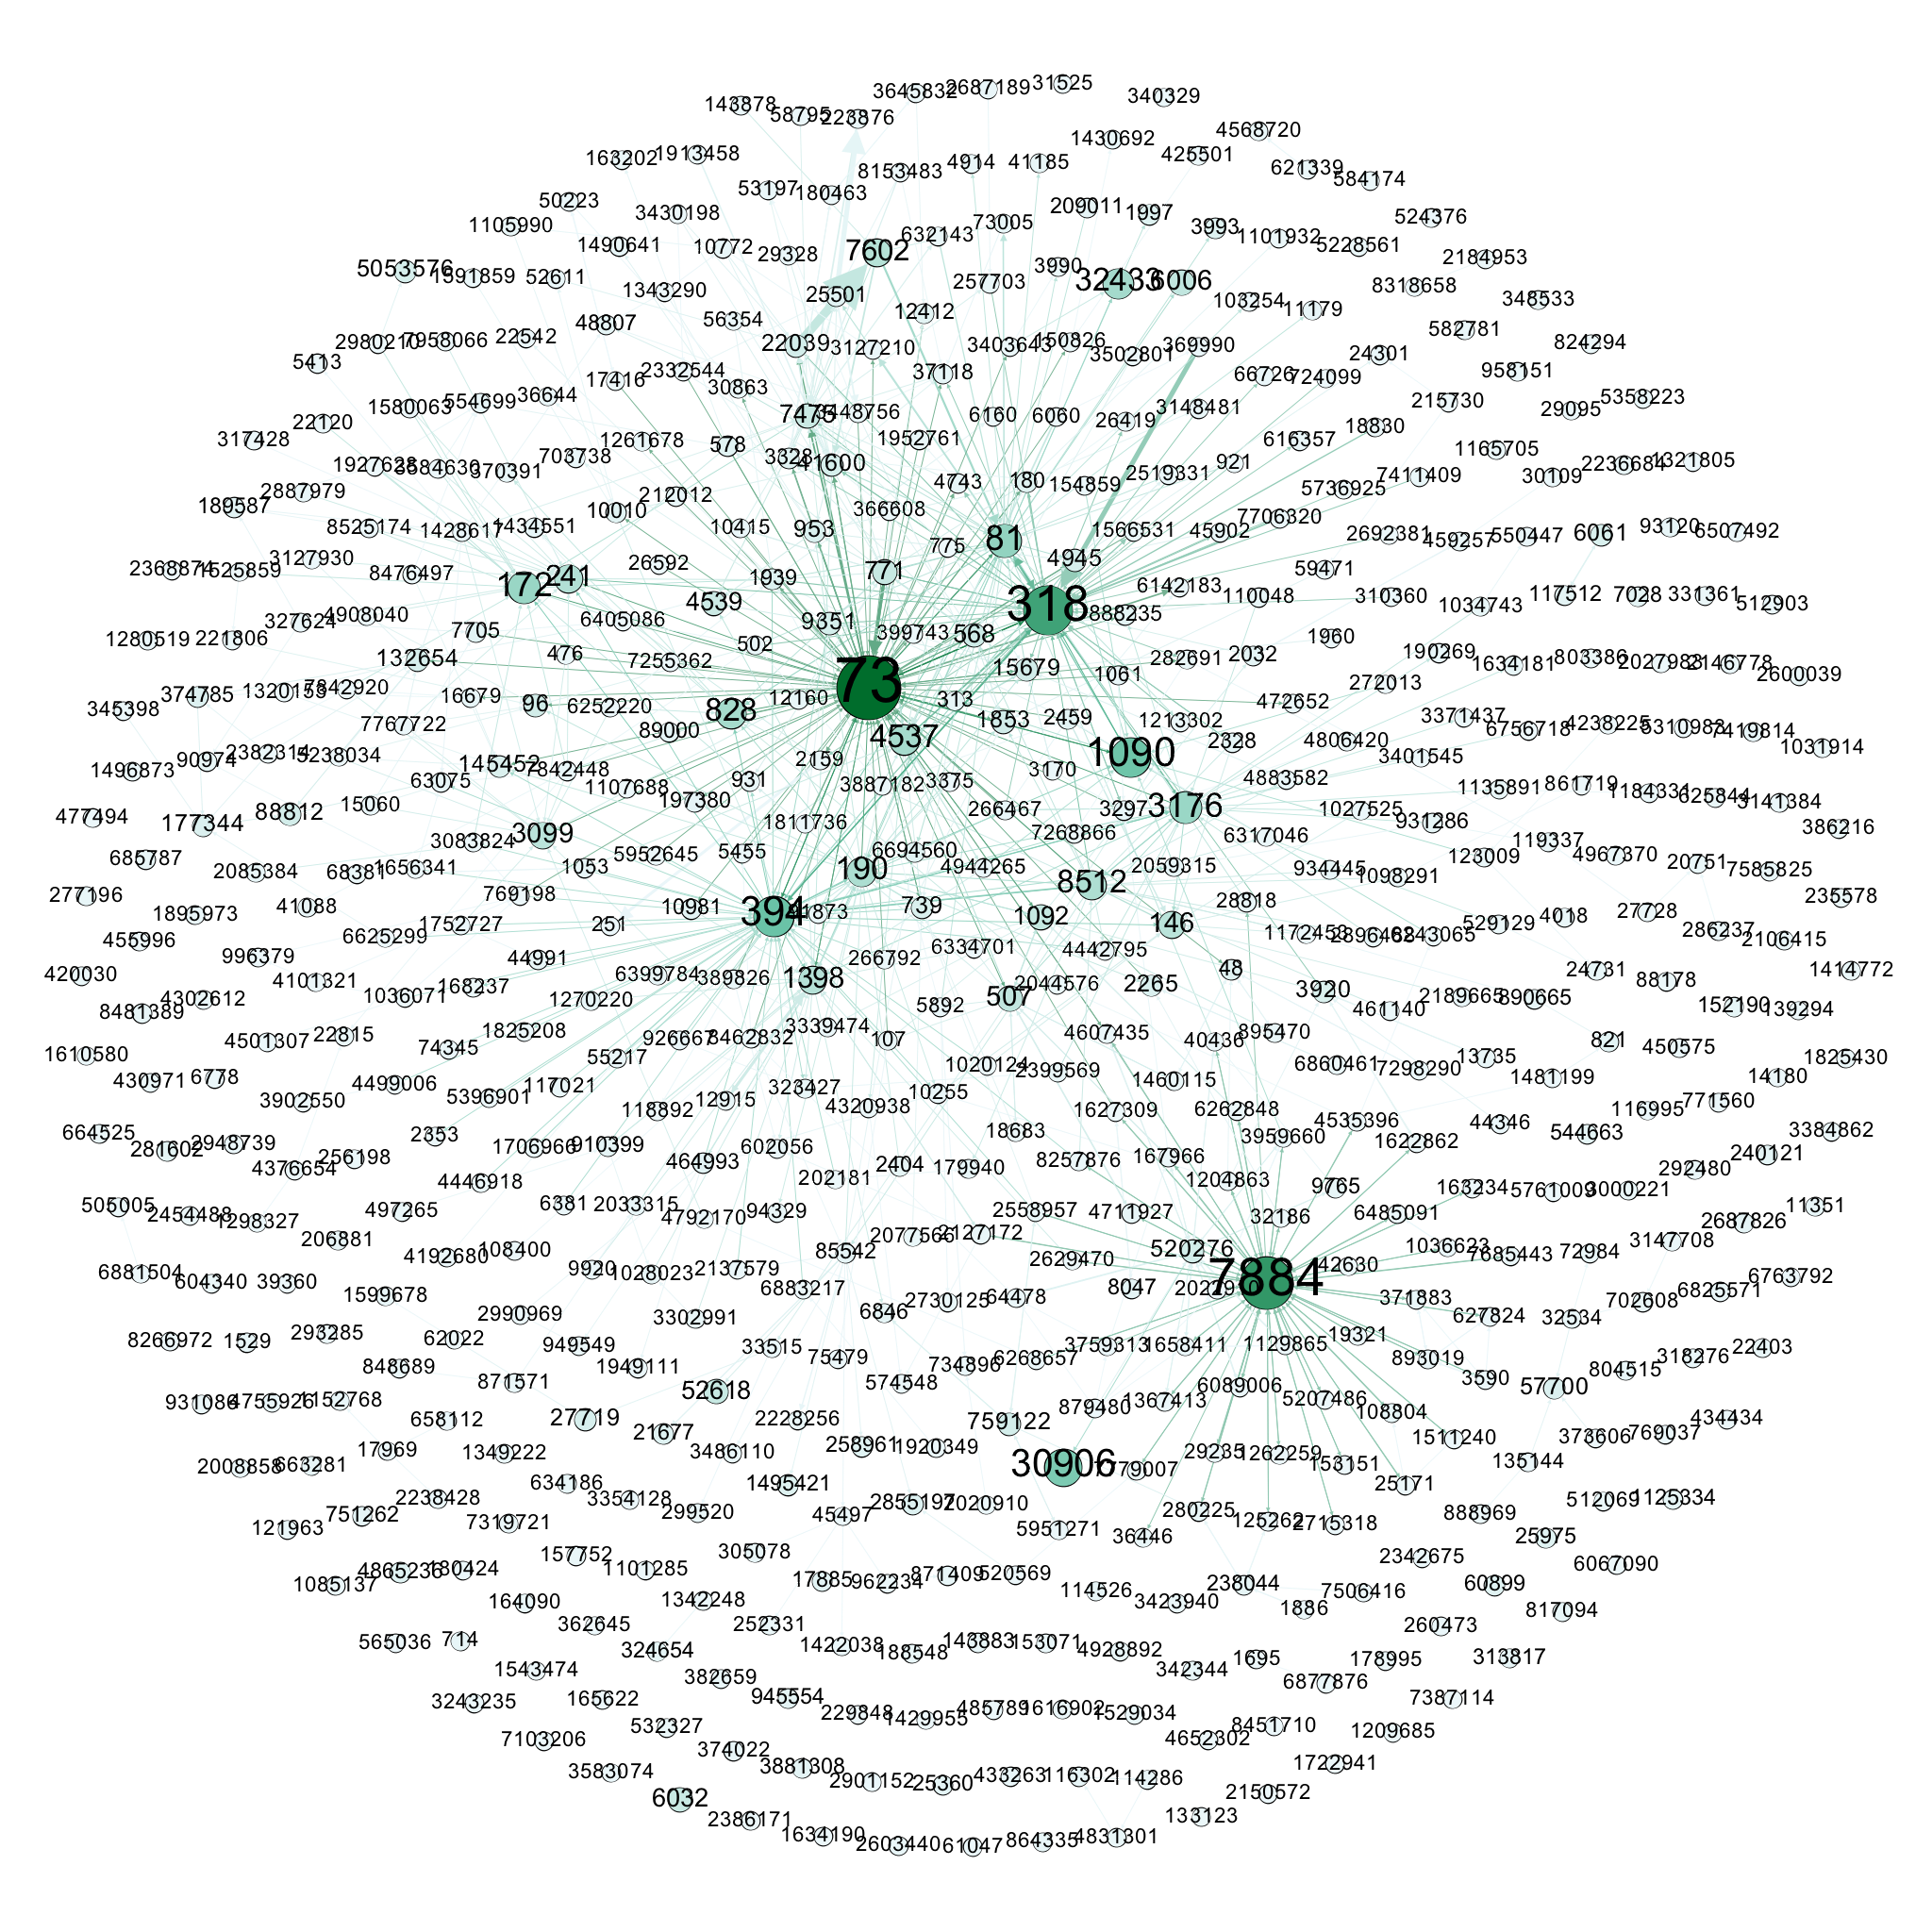
\includegraphics[width=\columnwidth]{viz} 
	\caption{The one day user graph on 25 Octobor 2013, filtered by the condition degree $\geq 6$. Each node is labelled by the user id and scaled by the pagerank score.} % The text in the square bracket is the caption for the list of figures while the text in the curly brackets is the figure caption
	\label{viz}
\end{figure}


\section{Prepartion for Security Analysis}

\subsection{Web Scraping}

In order to link the real world entities with bitcoin public keys, we scraped the bitcoin forum, bitcointalk.
Often, users will leave their public keys for donations in the signature of the forums. The example screenshot is shown in figure \ref{shot}.

\begin{figure}[h]
	\centering 
	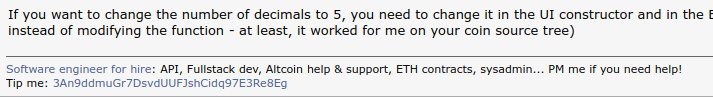
\includegraphics[width=\columnwidth]{address} 
	\caption{Screenshot of the user leaving their addresses in the forum post} % The text in the square bracket is the caption for the list of figures while the text in the curly brackets is the figure caption
	\label{shot}
\end{figure}

We used Beautiful Soup to scrape the pages and build the crawler. The crawler ran around 40 hours. 
Using breadth-first search we crawled around 5 links deep from the home pages. 
We parsed the signature section of each post and retrieved the public key through regular expression like $\Sigma \left\lbrace 26,33\right\rbrace $ where $\Sigma$ is a set of valid alphanumeric characters.
For each regular expression match, we ran the checksum function to validate it as a public key.
We finally retrieved around 3000 addresses by crawling around 50000 posts.

\subsection{Pagerank}

We applied PageRank algorithm to rank the user nodes in the order of importance.
This may be used to understand how those forums users are linked with the nodes with high importance.
Figure \ref{pr} shows top 10 users from pagerank.
The user 7884 belongs to SatoshiDICE, a gambling site.

\begin{figure}[h]
	\centering 
	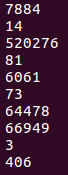
\includegraphics[width=0.2\columnwidth]{pagerank} 
	\caption{Top 10 users with high pagerank outputs. Most of the top ranked users were found to be gambling.} % The text in the square bracket is the caption for the list of figures while the text in the curly brackets is the figure caption
	\label{pr}
\end{figure}

\section{Case Study: Fraud Detection of Silk Road Arrest}

Posted on April 25, 2011, the user altoid accidently revealed their address.

\begin{figure}[!htb]
	\centering 
	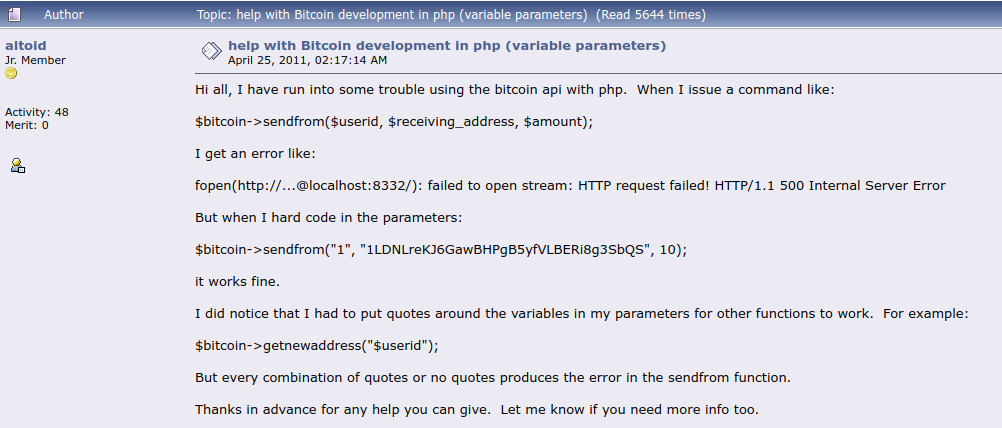
\includegraphics[width=\columnwidth]{post} 
	\caption{Post of the user altoid who accidently revealed their address on a forum post} % The text in the square bracket is the caption for the list of figures while the text in the curly brackets is the figure caption
	\label{post}
\end{figure}

We verified the address \textbf{“1LDNLreKJ6GawBHPgB5yfVLBERi8g3SbQS”} and found out that it was one of the highly ranked node of the pagerank output for that particular user node.
The user was revealed to be \textbf{"Dread Pirate Roberts"} who was involved in money laundering for the Silk Road fraud. FBI arrested him in 2013.

Using our bitcoin transaction graph, we found an address \\
\textbf{“1933phfhK3ZgFQNLGSDXvqCn32k2buXY8a”} which has \textbf{111,114.65 BTC} with nothing spent, shown in figure \ref{spent}.

\begin{figure}[h]
	\centering 
	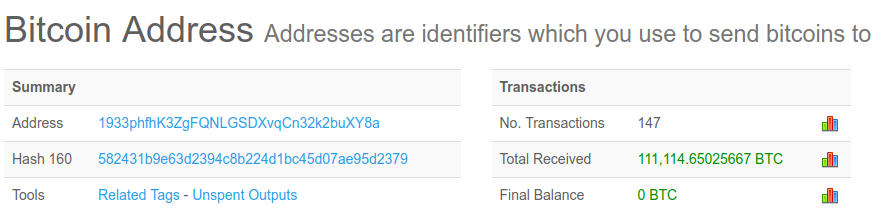
\includegraphics[width=\columnwidth]{spent} 
	\caption{This user has around 1000 million US dollars in the wallet, but they have spent nothing. We found this using the visualization of the flow of our design of bitcoin transaction graph,} % The text in the square bracket is the caption for the list of figures while the text in the curly brackets is the figure caption
	\label{spent}
\end{figure}

An interesting question, \textbf{is this address related to DPR’s address?}
We found that this address was in the same component as the user altoid’s component.
\textbf{Can we discover a trail for this address to reveal what addresses he used for coin mixing?}

We applied Djikstra’s algorithm between these two nodes to discover the shortest path. Hence, this could be trail he used to mix the coins and store them.
The final result of the trail is shown in figure \ref{trail}.

\begin{figure}[h]
	\centering 
	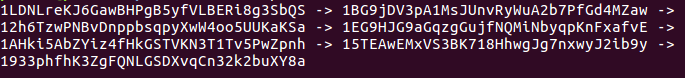
\includegraphics[width=\columnwidth]{trail} 
	\caption{Trail discovered from user's address to the public key of the wallet having a sketchy transaction.} % The text in the square bracket is the caption for the list of figures while the text in the curly brackets is the figure caption
	\label{trail}
\end{figure}

\section{Conclusions}
Bitcoin architecture is not entirely robust to the completely anonymous transactions.
Multi-input heuristics could be used to cluster the users from public key addresses. 
We presented a novel edge bundling algorithm on how transactions could be annotated to users by making use of this heuristic.
We have demonstrated that the exponentially growing data of bitcoin blockchain can still be parsed by a personal computer using our memory efficient algorithm.
We proved empirically that bitcoin graphs are indeed decentralized.
We presented some visualization to analyze the transaction flow and users of high importance.
We applied our findings on Silk Road arrest and our algorithms were able to detect the coin-mixing trail used by the deceiver.



\bibliographystyle{apalike}
\bibliography{paper}

\end{document}
